\documentclass[english]{article}

\usepackage{babel}
\usepackage{graphicx}
\usepackage{alltt}
\usepackage{url}
\usepackage{tabularx}
%\usepackage{ngerman}
\usepackage{longtable}
\usepackage{color}
\usepackage{framed}
\usepackage{array}

\usepackage{xifthen}
\newboolean{showbackdoors}
\setboolean{showbackdoors}{true}  % set to false to hide subsection on backdoors for reviewing group


\newenvironment{prettytablex}[1]{\vspace{0.3cm}\noindent\tabularx{\linewidth}{@{\hspace{\parindent}}#1@{}}}{\endtabularx\vspace{0.3cm}}
%\newenvironment{prettytable}{\prettytablex{l X}}{\endprettytablex}

\newcolumntype{L}{lp{0.3\textwidth}p{0.3\textwidth}p{15pt}p{15pt}p{15pt}}

\title{\huge\sffamily\bfseries System Description and Risk Analysis}
\author{B\"ahler Alessio \and Enz Andreas \and Niederberger Matthias}
\date{\today}


\begin{document}
\maketitle

%% **** please observe the page limit **** 
%% (it is not allowed to change the font size or page geometry to gain more space)
%% comment or remove lines below before hand-in
\begin{center}
{\large\textcolor{red}{Page limit: 30 pages.}}
\end{center}
%%%%%%%%%%%%%%%%%%%%%%%%%%%%%%%%%%%%%%%%%%%%%%

\tableofcontents
\pagebreak

\begin{framed}
\noindent
{\it
Recall the following guidelines when writing your reports:
\begin{itemize}
\item Adhere to the given templates.

\item Refer to the security principles in the book for justification.

\item Use clear terminology: 
\begin{itemize}
\item secure = confidential + authentic. Be clear about
which properties you are writing.
\item Are pairwise distinct: certificate, private key, public key, archive to of certificate with private key. Please avoid mixing these up.
\end{itemize}

\item Refer to the source document of your risk definitions if appropriate.

\item For the risk evaluation, formulate the threats in active, not passive, 
voice: who (threat source) does what (threat action)? 

\item Use a spell checker before hand-in!

\end{itemize}
}
\end{framed}


\section{System Characterization}

\subsection{System Overview}

%%% Describe the systems mission,  the system boundaries,
%%% and the overall system architecture, including the main subsystems and
%%% their relationships.   This description should provide a high-level
%%% overview of the system, e.g., suitable for managers, that complements
%%% the more technical description that follows.

The aim of this system is to provide the customer company with an in-house certificate authority (CA). This CA provides
employees with digital certificates on demand, which are used to secure email communication. 
The System consists of three machines in a company network and external client machines that connect over the Internet. 
Inside the company network we have Machine 1 housing the Core CA functionality and the legacy MySQL database. This means
that the main signing key and certificate revocation list (CLR) are stored and maintained on Machine 1. %How is main key stored? Where is CLR published? 
Machine 2 contains the web server with a firewall to shield it and the company network because any traffic from the 
Internet will have to cross the web server machine anyway. Finally Machine 3 is used for the physical separation of the 
backup service, with backup daemons connecting to the other two machines. 



\begin{figure}[htb!]
\centering{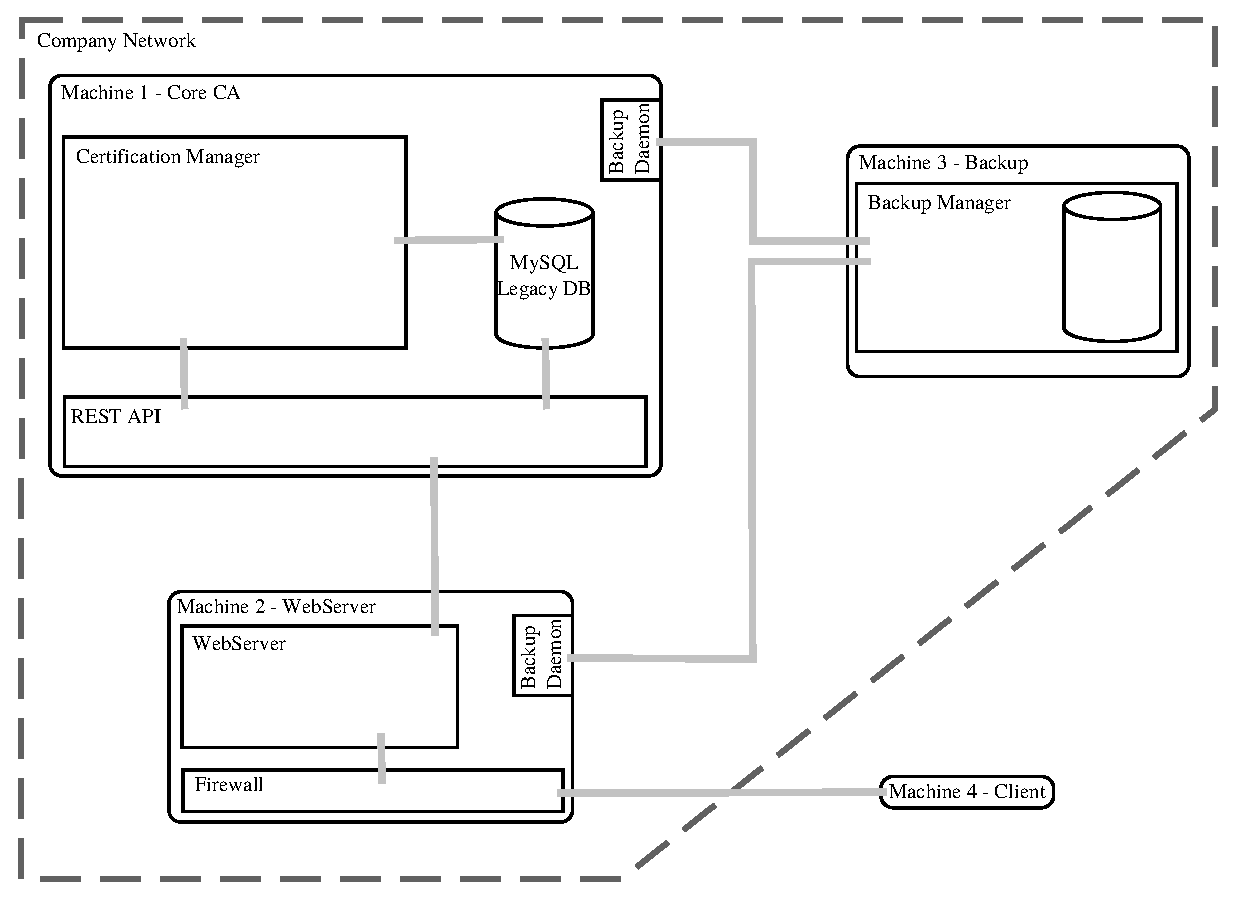
\includegraphics[width=\textwidth]{res/system_arch.eps}}
\caption{System Architecture of the company network including an external client machine.}
\centering
\label{fig:system_arch}
\end{figure}


\subsection{System Functionality}

Describe the system's functions.


\subsection{Security Design}

Describe the system's security design, including access control, key and session management,  and security of data at rest and in transit.


\subsection{Components}

%%% List all system components and their interfaces, subdivided, for example, into
%%%   categories such as platforms, applications, data records, etc. For
%%%   each component, state its relevant properties.

A short description of the components in Figure \ref{fig:system_arch}.

\begin{itemize}
    \item \textbf{Certification Manager}: Manages certificate state (creation, revocation, deletion, ...). Interfaces with the Web Server over the REST API and directly with the legacy MySQL database. It has two main subcomponents:
    \begin{itemize}
        \item Certification Store: A directory where keys and certificates are stored.
        \item Certification Generator: Built with OpenSSL
    \end{itemize}
    \item \textbf{MySQL DB}: As provided. Interfaces with the web server over a REST API and with the Certification Manager.
    \item \textbf{REST API}: Interface between Core CA machine and WebServer machine.
    \item \textbf{Web Server}: Accepts web traffic filtered through a firewall. Does authorization by checking legacy database and can request certificate state changes from the Certification Manager.
    \item \textbf{Firewall}: Filters traffic.
    \item \textbf{Backup Manager}: Periodically stores specified data in the backup database. Interfaces with Core CA and Web Server machine.
    \begin{itemize}
        \item Backup Daemon: Sends data to backup machine
    \end{itemize}
\end{itemize}


\ifthenelse{\boolean{showbackdoors}}{
% show for handed-in version

\subsection{Backdoors}

Describe the implemented backdoors. 

\bigskip\noindent
\textbf{Hide this subsection in the version handed over to the reviewing team by setting the flag \texttt{showbackdoors} at the top of this document to \texttt{false}.}


%% do not delete the three lines below
}{ 
% empty for reviewing group's version
} 

\subsection{Additional Material}

You may have additional sections according to your needs.


\section{Risk Analysis and Security Measures}

\subsection{Assets}

%% TODO: Describe the relevant assets and their required security
%%  properties. For example, data objects, access restrictions,
%%  configurations, etc.

\textbf{Physical Assets}
\begin{itemize}
\item Web Server: physical machine hosting the Web Server Application. Must be available and enable secure and tamper resistant communications with the clients.
\item Core CA: physical machine hosting the CA application and the legacy database.
\item Backup: physical machine hosting the backup data.
\item Internet Connectivity: Modem and lines connecting the WebServer to the Internet.
\item Internal Network: LAN via physical lines and a switching modem.
\end{itemize}

\noindent\textbf{Logical Assets}
\begin{itemize}
    \item Software
    \begin{itemize}
    \item Web Server Application
        \item Core CA Application
        \item Legacy MySQL database/application/driver?
        \item REST API
        \item Backup Daemon
        \item Backup Manager
        \item Firewall
    \end{itemize}
    \item Information
    \begin{itemize}
        \item Certificates
        \item Keys
        \item User data
        \item Configuration files
        \item Logs
    \end{itemize}
\end{itemize}


\noindent\textbf{Persons}
\begin{itemize}
\item System Administrator: maintains the system by applying software updates, controlling system logs to search malicious behaviours that could lead to security issues and ensuring that the machines hosting the systems components are working properly. He therefore has access to sensitive data, in the form of a remote connection well as physical access to all components.
\item CA Administrators: are able to verify the current state of the CA.
\item Users: Employees and Informants that both use the system to obtain certificates which allow them to communicate securely with the WebServer.
\item Management
\end{itemize}

\noindent\textbf{Intangible Goods}
\begin{itemize}
\item Company Reputation
\item Confidentiality of informant identities.
\end{itemize}

\subsection{Threat Sources}

% TODO: Name and describe potential threat sources (\emph{not} threats!) including their motivation.

\begin{itemize}
\item Nature: Floods, lightning strikes, earthquakes can damage the physical infrastructure.
\item Users: Employees (includes also cleaning personnel etc.) and informants can act maliciously or be careless/poorly trained.
\item Competitors: may be interested in obtaining confidential information to gain an advantage, blackmail or cause harm by publishing it. May resort to Skilled Hackers to achieve their goals.
\item "Victims": subjects of investigative reports that were publicly exposed and may want to get revenge by causing any kind of damage. May resort to Skilled Hackers to achieve their goals.
\item Organized Crime: can directly or indirectly be "Victim", could be interested in blackmailing the Company to gain money or just to obtain important information that can be sold on the black market/used for other illegal activities.
\item Malware: may be non-directional or self-spreading and have different goals, e.g. Ransomware, Trojans.
\item Expert Hackers: A skilled hacker has expert knowledge for some systems. He can write his own code and may use unknown or unpublished vulnerabilities (from book). May itself be a "Victim" or act for monetary interests.
\item Script Kiddies: This type of adversary has basic computer knowledge and uses mainly known vulnerabilities for which exploits are available on the Internet. However, he might write scripts to automate tasks or use tools to automatically create malware. His main motivations are challenge, glory and destruction (from book).
\item Organizatorial Deficiencies: lack in employee training, poor/non-existing/non-enforced security measures, such as unsanitized user input, can weaken the overall security of the system.
\item Hardware Failures
\end{itemize}

\subsection{Risks Definitions}

Definition of Likelihood, Impact and Risk level using the following three
  tables from \cite{ASL_book}.

%\subsubsection{Tools}

\begin{center}
\begin{tabular}{|l|p{0.8\textwidth}|}
\hline
%\multicolumn{2}{|c|}{\bf Likelihood} \\
%\hline
Likelihood & Description \\
\hline
\hline
High   & The threat source is highly motivated and sufficiently capable of exploiting a given vulnerability in order to change the asset's state. The controls to prevent the vulnerability from being exploited are ineffective. \\
\hline
Medium & The threat source is motivated and capable of exploiting a given vulnerability in order to change the asset's state, but controls are in place that may impede a successful exploit of the vulnerability. \\
\hline
Low   & The threat source lacks motivation or capabilities to exploit a given vulnerability in order to change the asset's state. Another possibility that results in a low likelihood is the case where controls are in place that prevent (or at least significantly impede) the vulnerability from being exercised. \\
\hline
\end{tabular}
\hspace{3em}
\begin{tabular}{|l|p{0.8\textwidth}|}
\hline
\multicolumn{2}{|c|}{\bf Impact} \\
\hline
Impact & Description \\
\hline
\hline
High   & The event (1) may result in a highly costly loss of major tangible assets or resources; (2) may significantly violate, harm, or impede an organization's mission, reputation, or interest; or (3) may result in human death or serious injury. \\
\hline
Medium & The event (1) may result in a costly loss of tangible assets or resources; (2) may violate, harm, or impede an organization's mission, reputation, or interest, or (3) may result in human injury. \\
\hline
Low   & The event (1) may result in a loss of some tangible assets or resources or (2) may noticeably affect an organization's mission, reputation, or inter- est. \\
\hline
\end{tabular}
\end{center}

\vspace{5mm}

\begin{center}
\begin{tabular}{|l|c|c|c|}
\hline
\multicolumn{4}{|c|}{{\bf Risk Level}} \\
\hline
{{\bf Likelihood}} & \multicolumn{3}{c|}{{\bf Impact}} \\ %\cline{2-4}
     & Low & Med & High \\  \hline
 High & Low & Med & High  \\
\hline
 Med & Low & Med & Med \\
\hline
 Low & Low & Low & Low \\
\hline
\end{tabular}
\end{center}



\subsection{Risk Evaluation}

% List all potential threats and the corresponding countermeasures. Estimate the risk based on the information about the threat, the threat sources and the corresponding countermeasure. Adhere to the risk definitions you have given above. As a sanity check, there should be at least one high-risk entry.

Potential threats and countermeasures with the inferred risk.


\subsubsection{{\it Evaluation Web Server}}

\begin{footnotesize}
\begin{prettytablex}{L}
No. & Threat &  Countermeasure(s) & L & I & Risk \\
\hline
1 & Expert Hackers: mount MitM attack to spy on and tamper with communications between Clients and WebServer. This allows the hackers to learn in particular a user's password and private keys. & HTTPs connection with Server side authentication & {\it Med} & {\it High} & {\it Med} \\
\hline
2 & Victim: resorts to Script Kiddies to launch DDoS attack on WebServer and cause damage, disruptions, maybe even ask money to stop & Simple DDoS protection like SYN cookies against syn flood & {\it High} & {\it High} & {\it High} \\
\hline
\end{prettytablex}
\end{footnotesize}

\subsubsection{{\it Evaluation Core CA}}

\begin{footnotesize}
\begin{prettytablex}{L}
No. & Threat &  Countermeasure(s) & L & I & Risk \\
\hline
1 & Hardware Failures: cause damages to the hard drives and privite CA key and certificate can't be recovered. &  & {\it Low} & {\it Med} & {\it Low} \\
\hline
\end{prettytablex}
\end{footnotesize}

\subsubsection{{\it Evaluation Backup}}

\begin{footnotesize}
\begin{prettytablex}{L}
No. & Threat &  Countermeasure(s) & L & I & Risk \\
\hline
1 & User: exploits physical access to Backup Machine and obtains backup data. & Physical protection of System Components, Disk Encryption & {\it Low} & {\it Med} & {\it Low} \\
\hline
\end{prettytablex}
\end{footnotesize}

\subsubsection{{\it Evaluation System Administrator}}

\begin{footnotesize}
\begin{prettytablex}{L}
No. & Threat &  Countermeasure(s) & L & I & Risk \\
\hline
1 & Expert Hacker: steals System Administrator credentials & Enforce Strong Passwords, Increase security sensibilization/awareness & {\it Med} & {\it High} & {\it Med} \\
\hline
2 & Organizatorial Deficiencies: illness or injury impede its work and the System is left unattended in case of problems/attacks & Good Documentation and making sure that not only one person knows the system & {\it High} & {\it Med} & {\it Med} \\
\hline
\end{prettytablex}
\end{footnotesize}

\begin{thebibliography}{---}
\bibitem[1]{CompSec} Computer Security: Principles and Practice. William Stallings and Laurie Brown, Prentice Hall, 2008
\bibitem[2]{ASL_book} Applied Information Security: A Hands-on Approach, David Basin, Patrick Schaller and Michael Schl�pfer, Springer, 2011
\end{thebibliography}

\end{document}

%%% Local Variables: 
%%% mode: latex
%%% TeX-master: "../../book"
%%% End: 
